% \begin{frame}[fragile]
% 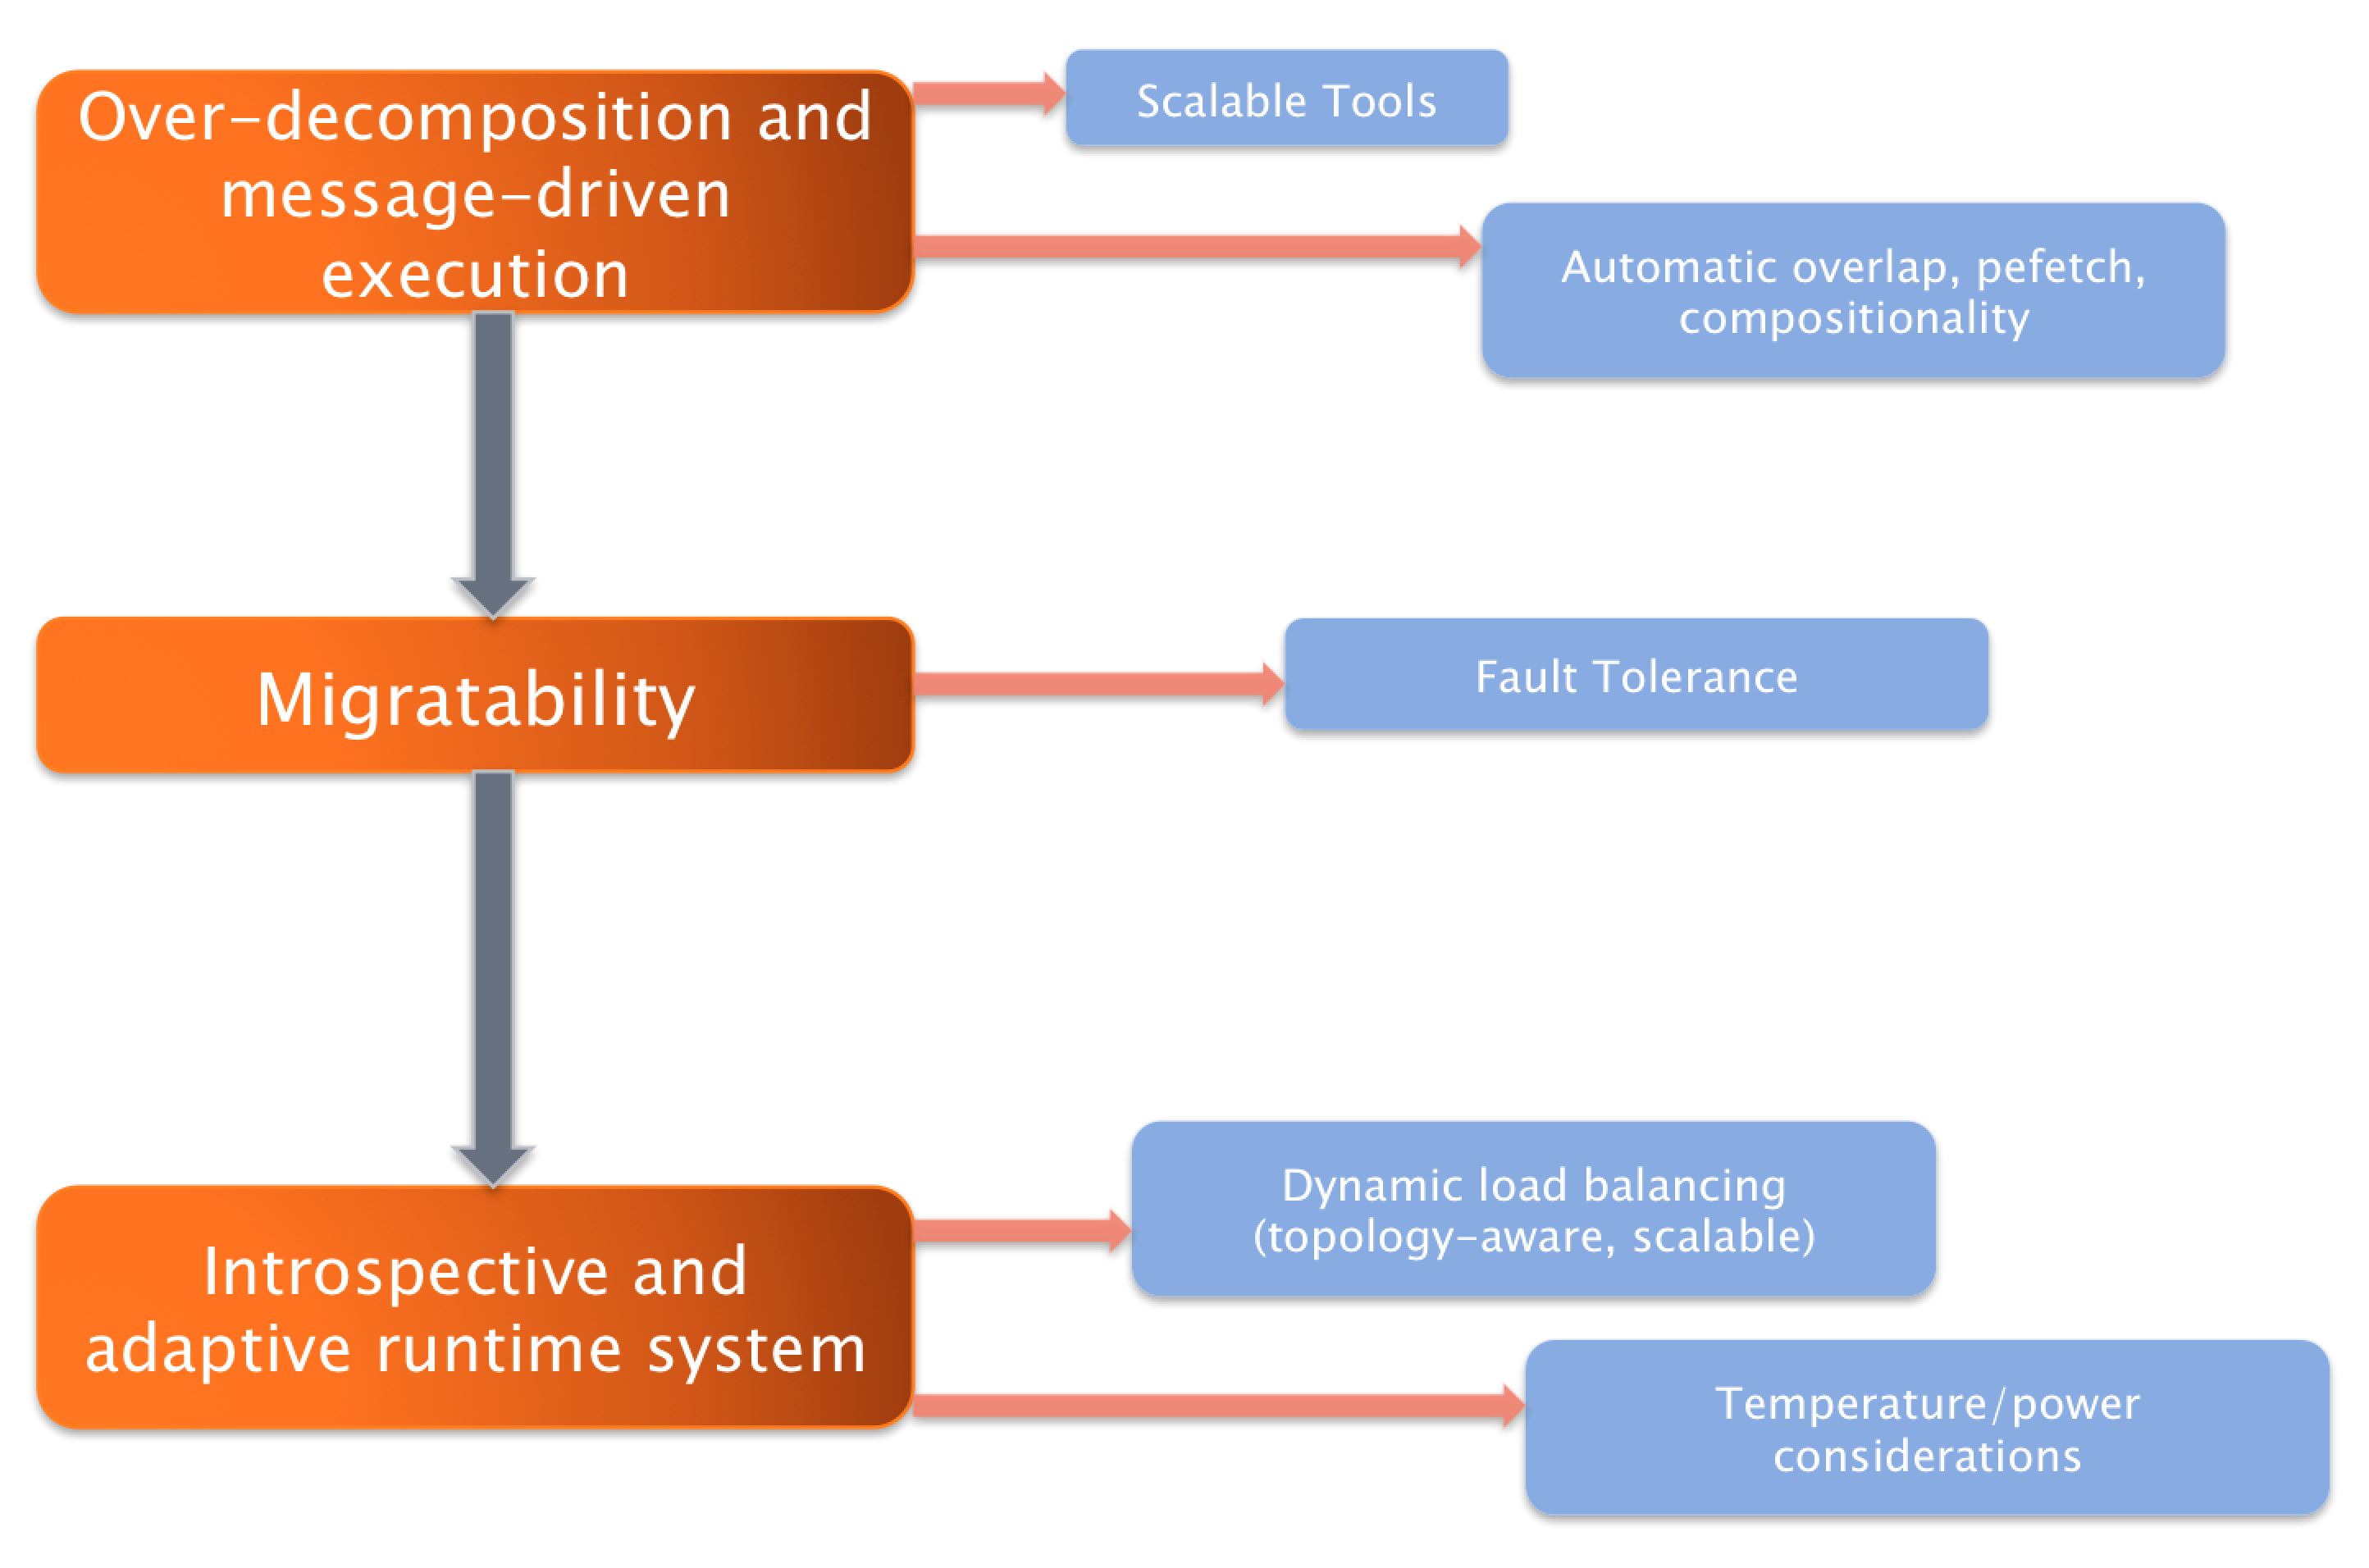
\includegraphics[width=0.9\textwidth]{figures/charmOutline.png}
% \end{frame}

\begin{frame}[fragile]
\frametitle{Load Balancing}
\begin{itemize}
 \item Static
   \begin{itemize}
   \item Irregular applications
   \item Programmer shouldn't have to figure out ideal mapping
   \end{itemize}
 \item Dynamic
   \begin{itemize}
   \item Applications are increasingly using adaptive strategies
   \item Abrupt refinements
   \item Continuous migration of work: e.g. particles in MD
   \end{itemize}
 \item Challenges
   \begin{itemize}
   \item Performance limited by most overloaded processor
   \item The chance that one processor is severely overloaded gets higher as
     \#processors increases
   \end{itemize}
\end{itemize}
\begin{center}\textbf{Migratable Objects Empower Automated Load Balancing!}\end{center}
\end{frame}


% \begin{frame}[fragile]
% \frametitle{Principle of Persistence}
% \begin{itemize}
%  \item Once the computation is expressed in terms of its natural (migratable)
%    objects
%  \item Computational loads and communication patterns \emph{tend to} persist,
%    even in dynamic computations
%  \item So, recent past is a good predictor of near future
%  \item The runtime system mediates communication between objects, and schedules
%    execution of objects, so it can introspect: record computation loads and
%    communication graphs
% \end{itemize}
% \end{frame}


% \begin{frame}[fragile]
% \frametitle{A quick Example}
% \framesubtitle{Weather Forecasting in BRAMS}
% \begin{itemize}
%  \item Brams: Brazillian weather code (based on RAMS)
%  \item AMPI version (Eduardo Rodrigues, with Mendes and J. Panetta)
% \end{itemize}
% 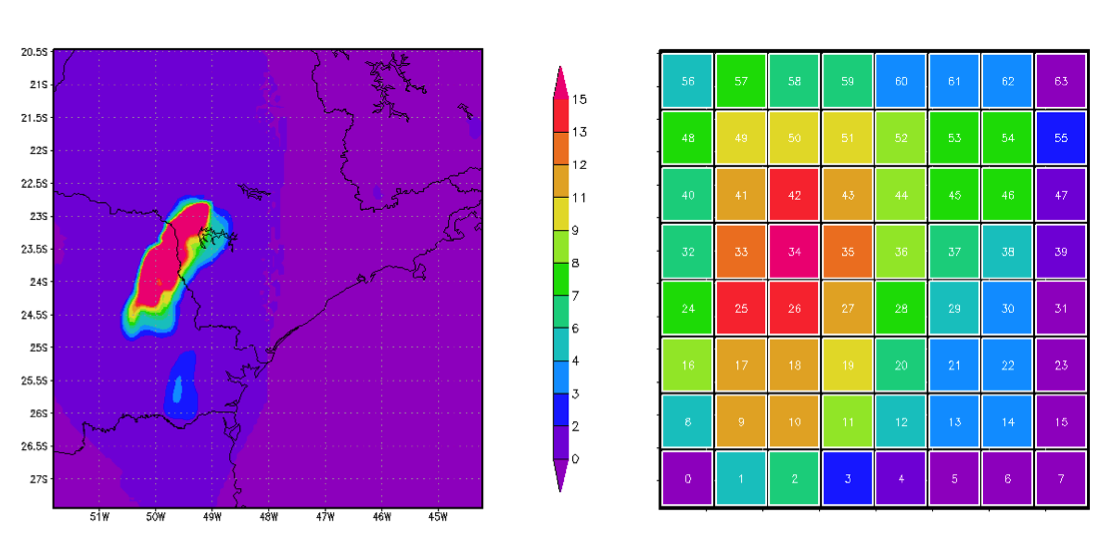
\includegraphics[width=0.9\textwidth]{figures/bramsVisual.png}
% \end{frame}


% \begin{frame}[fragile]
% \frametitle{Basic Virtualization of BRAMS}
% 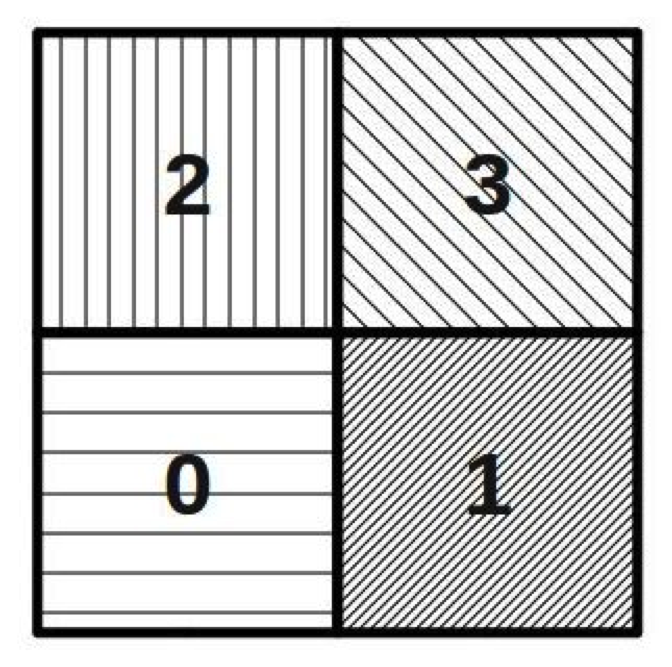
\includegraphics[width=0.5\textwidth]{figures/bramsNonVirtual.png}%
% 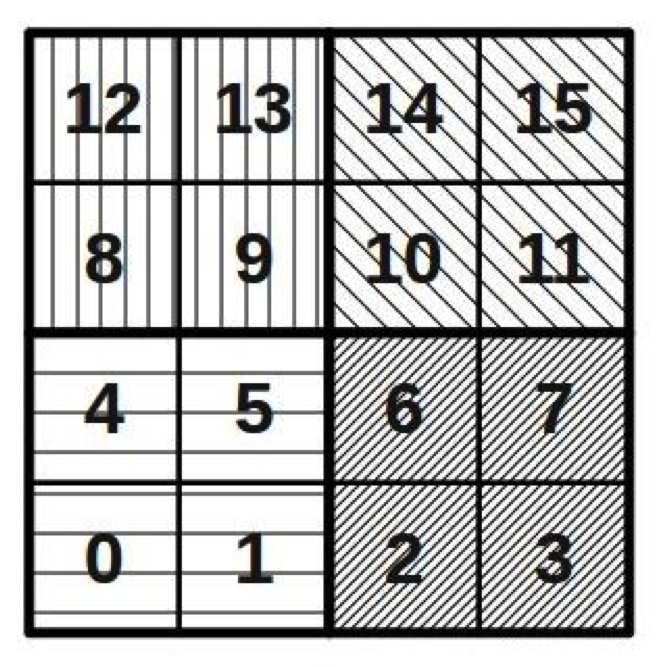
\includegraphics[width=0.5\textwidth]{figures/bramsVirtual.png}
% \end{frame}

% \begin{frame}[fragile]
% \frametitle{Baseline: 64 objects on 64 processors}
% \begin{center}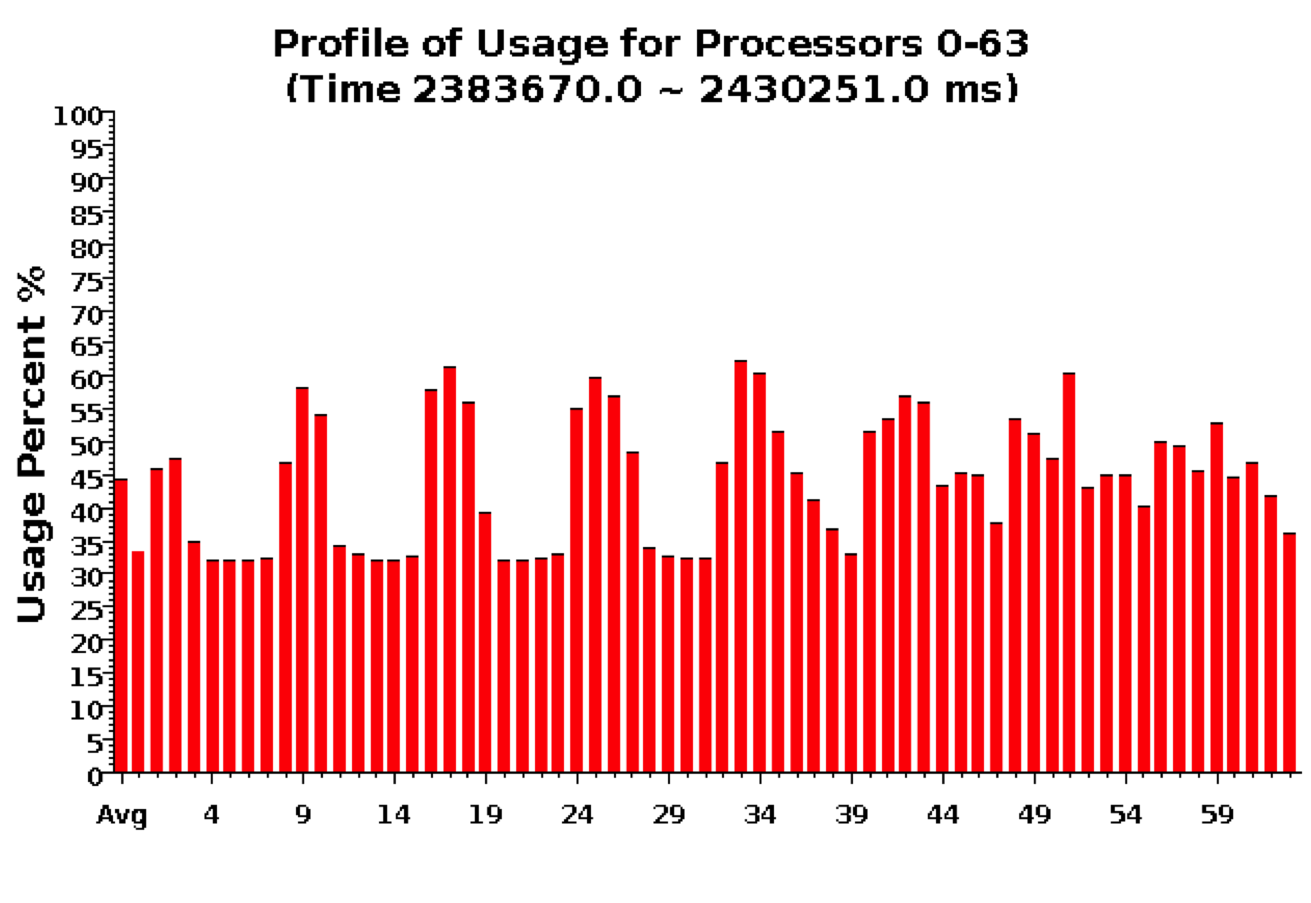
\includegraphics[width=0.9\textwidth]{figures/usageNonVirtual.png}\end{center}
% \end{frame}

% \begin{frame}[fragile]
% \frametitle{Over-decomposition: 1024 objects on 64 processors}
% \framesubtitle{Benefits from communication/computation overlap}
% \begin{center}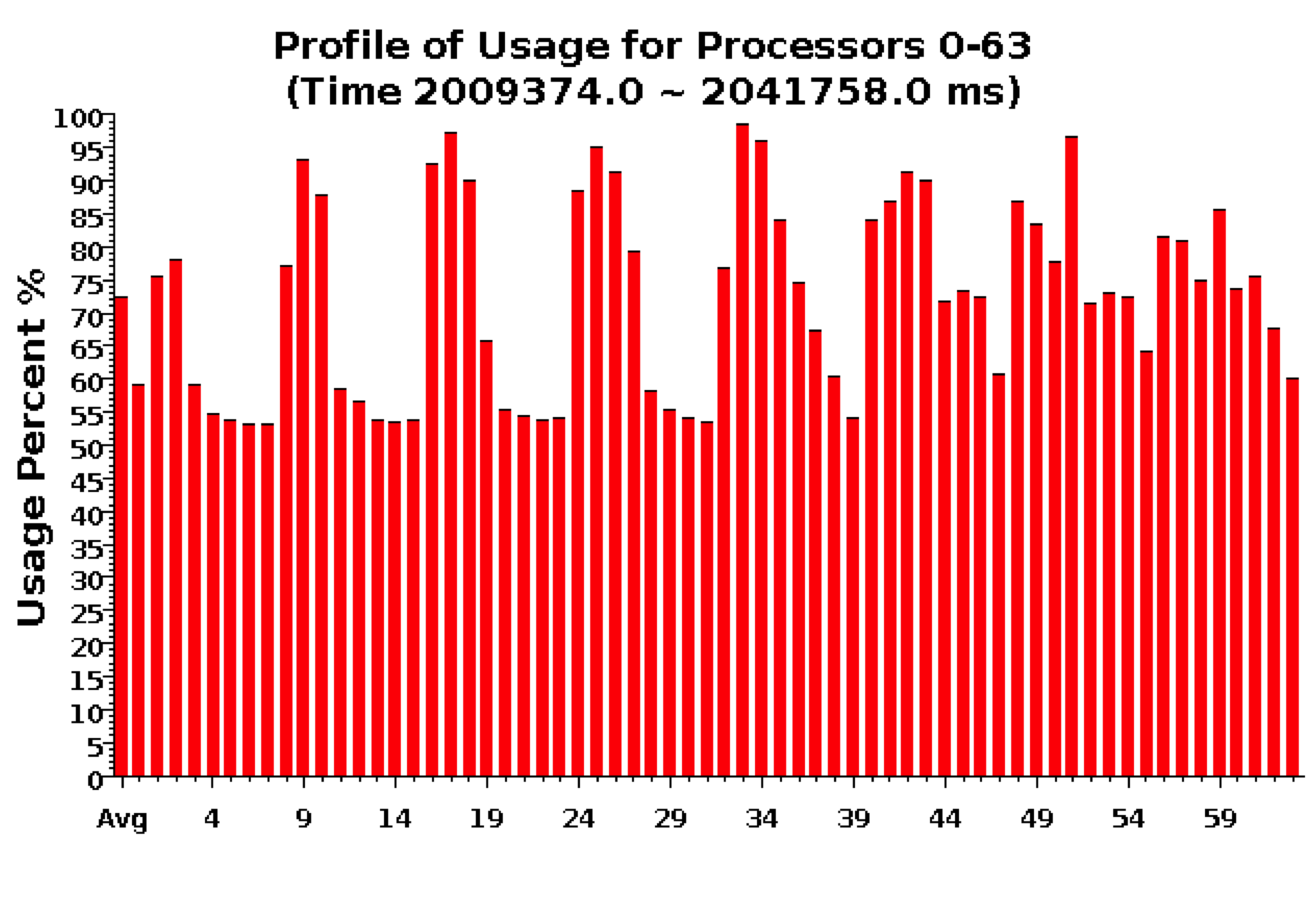
\includegraphics[width=0.9\textwidth]{figures/usageVirtual.png}\end{center}
% \end{frame}

% \begin{frame}[fragile]
% \frametitle{With Load Balancing: 1024 objects on 64 processors}
% \begin{center}
% \begin{itemize}
% \item No overdecomp (64 threads): 4988 sec
% \item Overdecomp into 1024 threads: 3713 sec
% \item Load balancing (1024 threads): 3367 sec
% \end{itemize}
% 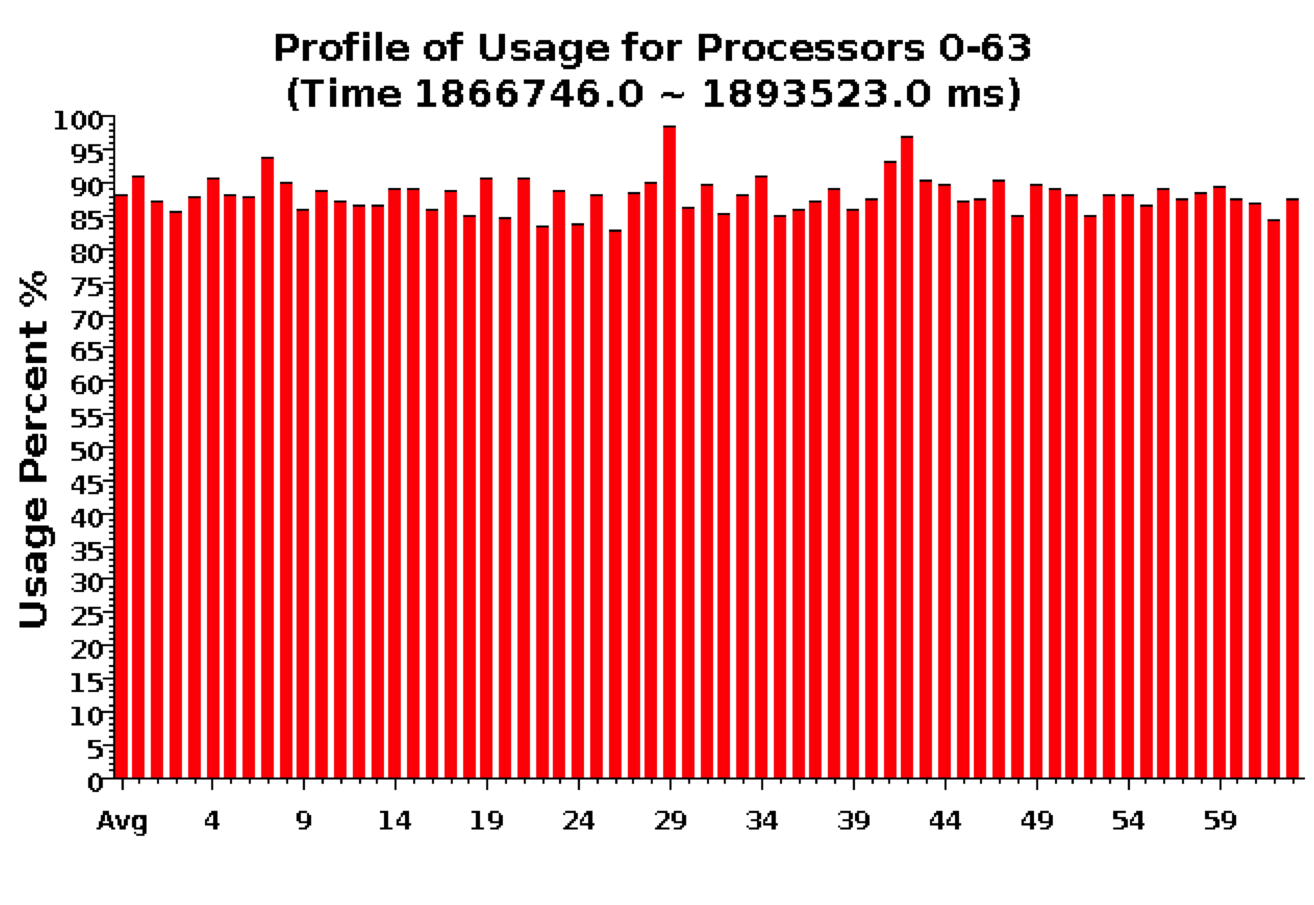
\includegraphics[width=0.8\textwidth]{figures/usageLB.png}
% \end{center}
% \end{frame}
